\documentclass[12pt,a4paper,utf8x]{report}
\usepackage{lmodern}
\usepackage[T1]{fontenc} 
\usepackage[utf8]{inputenc}  
\usepackage [frenchb]{babel}

% Pour pouvoir utiliser le verbatim dans les sections utiliser la commande versalitas
\newcommand{\versalitas}[1]{{\usefont{T1}{cmr}{bx}{sc}#1}}% 

\usepackage{textcomp}
\usepackage{keystroke}
\usepackage{amssymb}
 
\usepackage{amsmath}
\renewcommand{\thesection}{\arabic{section}} % numérotation des sectiosn
\usepackage[cc]{titlepic} %rajouter le logo dans la page de garde
\usepackage{url} % Pour avoir de belles url
\usepackage {geometry}
\usepackage[linktocpage]{hyperref}

% Pour mettre du code source
\usepackage {listings}
% Pour pouvoir passer en paysage
\usepackage{lscape}	

% Pour pouvoir faire plusieurs colonnes
\usepackage {multicol}

% POur crééer un index
\usepackage{makeidx}

\usepackage[pdftex]{graphicx}

\hypersetup{
backref=true,
%permet d'ajouter des liens dans...
pagebackref=true,%...les bibliographies
hyperindex=true, %ajoute des liens dans les index.
colorlinks=true, %colorise les liens
breaklinks=true, %permet le retour à la ligne dans les liens trop longs
urlcolor= blue, %couleur des hyperliens
citecolor=	cyan,
bookmarks=true, %créé des signets pour Acrobat
bookmarksopen=true,
%si les signets Acrobat sont créés,
%les afficher complètement.
pdftitle={Initiation à la Recherche}, %informations apparaissant dans
pdfauthor={MARGUERITE Alain\\ RINCE Romain},
%dans les informations du document
pdfsubject={Doc}
%sous Acrobat.
}
\hyphenation{si-tu-a-tion}
\makeindex

\newcommand\fractal{\textsc{Fractal}} 
\newcommand\julia{\textsc{Julia}} 
%%%% debut macro pour enlever le nom chapitre %%%%
% \makeatletter
% \def\@makechapterhead#1{%
%   \vspace*{50\p@}%
%   {\parindent \z@ \raggedright \normalfont
%     \interlinepenalty\@M
%     \ifnum \c@secnumdepth >\m@ne
%         \Huge\bfseries \thechapter\quad
%     \fi
%     \Huge \bfseries #1\par\nobreak
%     \vskip 40\p@
%   }}
% 
% \def\@makeschapterhead#1{%
%   \vspace*{50\p@}%
%   {\parindent \z@ \raggedright
%     \normalfont
%     \interlinepenalty\@M
%     \Huge \bfseries  #1\par\nobreak
%     \vskip 40\p@
%   }}
% \makeatother
%%%% fin macro %%%%

%Couverture 

%Couverture 
\widowpenalty=10000
\clubpenalty=10000
 
\title{{\Huge Résumé d'article}\\\vspace{1cm}An open component Model and its support in Java\\\vspace{0.3cm}
\small E. \textsc{Bruneton}*, T. \textsc{Coupaye}*, M. \textsc{Leclerc}**, V. \textsc{Quema}**, J.B. \textsc{Stefani}**\\
France Télécom R\&D* et \textsc{INRIA} Rhône-Alpes**}
\titlepic{
\includegraphics[scale=0.80]{img/logouniv}}
		

\author{Romain \textsc{Rincé}}
\date{Université de Nantes \\ 2 rue de la Houssinière, BP92208, F-44322 \textsc{Nantes} cedex 03, \textsc{France}}

\hyphenation{appar-tiennent}
\hyphenation{pro-blèmes}

\begin{document}

\maketitle
\renewcommand{\labelitemi}{$\bullet$} 

\clearpage

% \tableofcontents
\clearpage

\section{Introduction}
Le papier \og \emph{An open component Model and its support in Java}\fg{} présente le modèle à composant \fractal{} réalisé conjointement avec la section R\&D de France Télécom et l'équipe \textsc{INRIA} Rhône-Alpes. 

L'objectif des auteurs étant de résoudre un certain nombre de limitations présentes dans les différents modèles existants (e.g. \textsc{EJB}, \textsc{CORBA}, .Net) telles que :
\begin{itemize}
 \item Les faibles possibilités d'extensibilité.
 \item La difficulté (voire l'impossibilité) d'ajouter dynamiquement des moyens de contrôle sur les composants.
 \item La nécessité de parfois devoir faire des choix difficiles entre le degré de configurabilité et les performances. 
\end{itemize}
Afin de répondre à ces problématiques, les auteurs présentent leur modèle à composant \fractal, ainsi que son implémentation en Java, le framework \julia.




\section{Le modèle à composant \versalitas{Fractal}}
L'objectif du modèle à composants \fractal{} est de pouvoir implémenter ou gérer des systèmes logiciels complexes, et ce même sur des systèmes moins traditionnels tels que l'embarqué. Pour ce faire \fractal{} offre la possibilité d'avoir des composants composite, des composants partagés,  des capacités d'introspection et de reconfiguration.

Il est à présent nécessaire de détailler un peu plus précisément le modèle \fractal{} (c.f. Figure \ref{fig:Comp}). Le modèle \fractal{} est principalement composé de deux entités qui sont le contenu et la membrane. 
\begin{figure}[htbp] %on ouvre l'environnement figure
  \center
  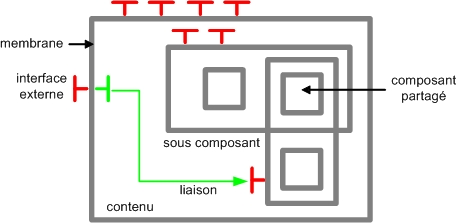
\includegraphics{img/fractal_component}
  \caption{Exemple d'un modèle \fractal{} de composants} %la légende
 \label{fig:Comp} %la légende
\end{figure}

\paragraph{Contenu}Le contenu peut être soit un ensemble de composants, soit du code du langage cible (e.g. Un objet en java).
\paragraph{Membrane} La membrane est l'élément qui permet au modèle d'offrir une organisation en composant. Celle-ci va encapsuler le contenu pour lui offrir les propriétés d'un composant. La membrane dispose en effet d'interfaces externes pour communiquer avec des composants de même niveaux ou avec son parent, et d'interfaces internes pour communiquer avec ses sous-composants. Ces interfaces peuvent être soit de type \verb+Client+ (c'est-à-dire qui demandent un service), soit de type \verb+Serveur+ (c'est-à-dire qui fournissent un service). Les interfaces \verb+Serveur+ peuvent être reliées à plusieurs interfaces \verb+Client+ ou aucune. Les interfaces des composants devant bien évidemment être liées pour pouvoir communiquer. 

La membrane dispose aussi de contrôleurs qui offrent un certain nombre d'actions sur le composant. Ces contrôleurs peuvent notamment effectuer les actions suivantes :
\begin{itemize}
 \item Accéder ou modifier les attributs du composant.
 \item Modifier les liaisons internes au composant.
 \item Ajouter ou supprimer des sous-composants.
 \item Agir sur le cycle de vie du composant (e.g. Démarrer ou arrêter l'exécution du composant).
\end{itemize}
Il s'agit bien sûr d'une liste non-exhaustive des contrôleurs ; le modèle \fractal{} permettant l'extensibilité de ses contrôleurs. 

Pour une spécification plus détaillée, vous pouvez vous reporter au rapport technique de \fractal\cite{TFCM}.






\section{Le framework \versalitas{Julia}}
\julia\cite{Julia} est un framework implémentant en Java le modèle \fractal. Il fournit donc un ensemble extensible de classes (\verb+Controller+ et \verb+Interceptor+) permettant le design des membranes des composants. L'objectif étant de répondre aux problématiques présentées en introduction, \julia{} permet une gestion des coûts en performance plus fine grâce à une continuité entre la reconfiguration statique et dynamique. De plus \julia{} doit pouvoir fonctionner sur des environnements restraints n'ayant, par exemple, pas de \verb+ClassLoader+, pas d'\textsc{API} de reflexion, pas d'\textsc{API} de collection~\dots{}

\paragraph{Présention}\julia{} dipose donc d'un ensemble de \verb+Controller+ et d'\verb+Interceptor+ (c.f. Figure \ref{fig:Julia} ).
\begin{figure}[htbp] %on ouvre l'environnement figure
  \center
  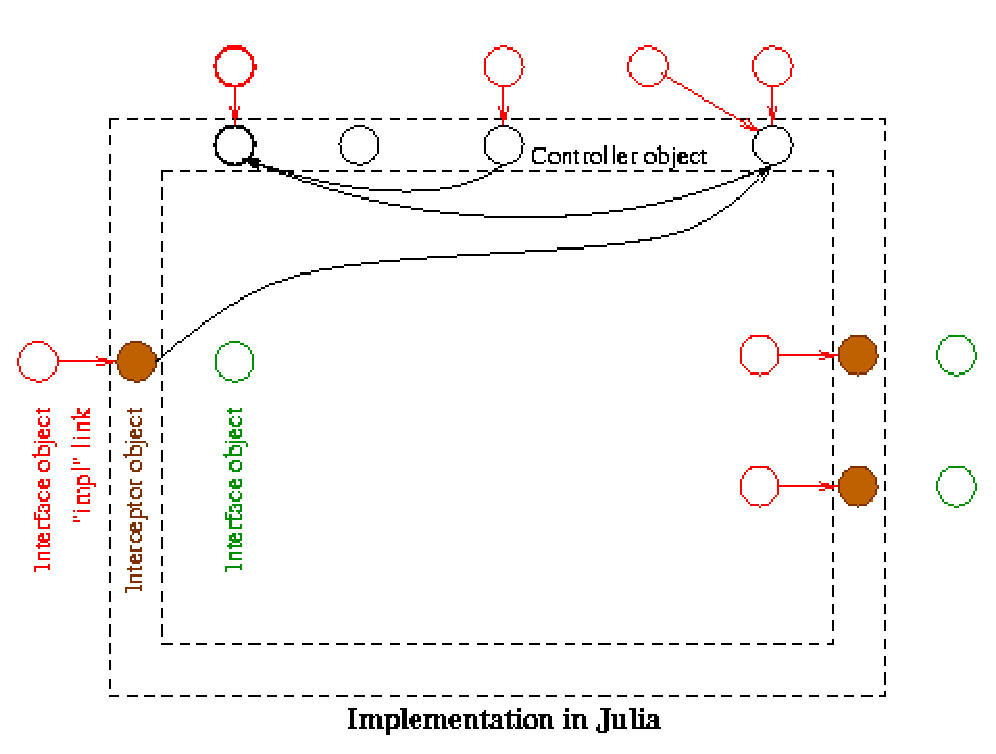
\includegraphics[scale=0.7]{img/implJ}
  \caption{Exemple d'un modèle \fractal{} de composants} %la légende
 \label{fig:Julia} %la légende
\end{figure} 
Les \verb+Interceptor+ gèrent les entrées/sorties sur l'appel de méthodes des interfaces (à l'exception des interfaces de contrôle). Les \verb+Controller+ quant-à-eux correspondent, en terme de concept, aux contrôlleurs de \fractal. Dans son ensemble un composant est donc un ensemble de trois types d'objets : 
\begin{itemize}
 \item Les objets qui implémentent les interfaces. Il faut noter qu'il est nécessaire de passer par un \verb+Interceptor+ pour que la membrane ait accès à cet objet concret (L'interface ayant un lien \verb+impl+ vers cet objet) ; les interfaces \verb+Client+ ont leur lien \verb+impl+ à \verb+null+ (Ils ne nécessitent pas d'objets les instanciants).
 \item Les objets de la membrane (\verb+Controller+ et \verb+Interceptor+).
 \item Les objets implémentants le contenu.
\end{itemize}

\paragraph{Extensibilité}Afin de permettre l'extensibilité de son framework, \julia{} fournit un mécanisme de classe abstraite permettant d'étendre les classes offertes de base. Par exemple il est possible d'étendre un contrôlleur gérant le démarrage et l'arrêt d'un composant (i.e. un \verb+LifeCycleController+) pour lui fournir une capacité d'arrêt automatique.

\paragraph{Optimisations}Pour améliorer les performances, \julia{} effectue divers optimisations
\begin{itemize}
\item Des optimisations intra-composant qui consistent à faire fusionner les objets de certains contrôleurs entre-eux. 
\item Des optimisations inter-composant qui consistant à effectuer des optimisations de référence sur les liens (c.f. Figure \ref{fig:short}).
\begin{figure}[htbp] %on ouvre l'environnement figure
  \center
  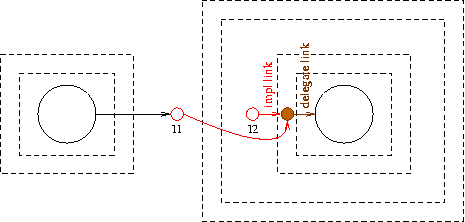
\includegraphics[scale=0.5]{img/shortcut}
  \caption{Exemple d'un modèle \fractal{} de composants} %la légende
 \label{fig:short} %la légende
\end{figure} 

\section{Qualité du modèle \versalitas{Fractal} et de \versalitas{Julia}}
Dans la dernière partie du papier, les auteurs évaluent leur travail par rapport aux problèmes soulevés en début de rapport. \julia{} semble répondre à toutes leurs exigences, tant sur le plan de la modularité et l'extensibilité, que sur les performances (notamment mémoire). De plus \julia{} étant relativement léger (45 ko en exécution), il est capable de tourner sur des systèmes extêmement restreints.

Cependant les auteurs soulèvent certaines limitations au niveau de la modularité et de l'exensibilité du framework \julia{} ; notamment dû au méchanisme de classes abstraites proposé.
\paragraph{Brève conclusion} 
Les résultats obtenus par les auteurs ainsi qu'une relative fierté de ces derniers vis-à-vis de leurs travaux, laissent à penser que le modèle \fractal{} possède nombre de qualités ; la création d'une communauté développant de nouveaux frameworks autour de celui-ci (AOKell\cite{AOKell}, Think\cite{Think}, FracTalk\cite{FracTalk}~\dots) ne fait que confirmer cette observation.
  
\end{itemize}

 %on ferme l'environnement figure
% Pour avoir un interligne de 1,5
% \input{P0}
%\input{P01}
% \input{P1}
% \input{P2}
% \input{annexereal}

% Pour finir l'interligne de 1,5

\printindex

\appendix
\bibliographystyle{alpha}
\bibliography{biblio.bib}

\end{document}
